\documentclass[a4paper,12pt]{article}
\usepackage[utf8]{inputenc}
\usepackage[brazilian]{babel}

\usepackage{mathptmx}               %Times New Roman
\usepackage{newtxtext,newtxmath} 

\usepackage{setspace}
\setstretch{1}      % Espacio entre lineas

\usepackage{vmargin}
\setpapersize{A4}
\setmargins{3cm}	% margen izquierdo
{1.5cm}            	% margen superior
{15cm}          	% anchura del texto
{23.5cm}          	% altura del texto
{10pt}             	% altura de los encabezados
{1cm}              	% espacio entre el texto y los encabezados
{0pt}              	% altura del pie de página
{1.5cm}             % espacio entre el texto y el pie de página

\usepackage{cite}

\usepackage{flushend}
\usepackage{amsmath}
\usepackage{textcomp}

\usepackage{multirow}

\usepackage[usenames]{color}
\usepackage[hidelinks]{hyperref} 

\usepackage{enumitem,kantlipsum}

\usepackage{graphicx} % figuras
\usepackage[export]{adjustbox}
\usepackage[labelfont=bf]{caption} %Negrita al label de la figura
\usepackage[font=it]{caption} %Italica descripcion de la figura 

\usepackage{fancyhdr,lipsum} %Encabezados
\pagestyle{fancy}
\setlength{\headheight}{52pt}

\fancypagestyle{plain}{
\fancyhead[L]{}
\fancyhead[R]{CAP-239-4 - Matemática Computacional 1}
\setlength{\headheight}{15pt}
\renewcommand{\headrulewidth}{0.5pt}}

\usepackage{subcaption}
\usepackage{breqn}

%% Algoritmos
\usepackage{algorithm}
\usepackage{amsmath}
\usepackage{algpseudocode}

\makeatletter
\def\BState{\State\hskip-\ALG@thistlm}
\makeatother

% Comando para facilitar a inserção de figuras
\newcommand{\image}[4]{
    \begin{figure}[H]%[h]
        \begin{center}
        \caption{#3}
        \includegraphics[scale=#1]{#2}
        \label{#4}
        \end{center}
    \end{figure}
}

\begin{document}
\begin{figure}
 \begin{center}
  
\includegraphics[width=1\linewidth]{fig/logoinpe.png}
 \end{center}
\end{figure}

\setlength{\textfloatsep}{0pt}

\title{Relatório final \\ Análise Estatística e Espectral de Processos Estocásticos}

\author{Fernando Cossetin, Felipe Menino, Felipe Perin}
\date{}

\maketitle

\section{Introdução}

% Assuntos a serem tratados na introdução:
% \begin{itemize}
%     \item Pandemia;
%     \item Análise estatística e espectral de processos estocásticos;
%     \item Objetivo do trabalho;
%     \item Técnicas aplicadas.
% \end{itemize}

\par O mundo passa por um período diferente, estamos sob efeito de uma enfermidade epidêmica amplamente disseminada, comumente conhecida como pandemia. Este quadro se dá pela presença de uma doença infecsiosa denominada COVID-19, causada pela infeção com o coronavírus da síndrome respiratória aguda grave 2 (SARS-CoV-2). O vírus transmite-se através de gotículas produzidas nas vias respiratórias das pessoas infetadas e com isso é altamente transmissível. Medidas foram e estão sendo tomadas no intúito de barrar essa disseminação e a que mais se mostrou eficaz foi o isolamento social. Ao mesmo tempo em que o isolamento é benéfico, é prejudicial no quesito econômico e isso tem gerado diversos impasses, até mesmo governamentais. Logo, a análise estatística estocástica, associada à variáveis aleatórias independentes se mostra uma ferramenta extremamente útil no processo de compreensão de como a pandemia está se comportando e com isso tentar prever o que está por vir.

\par Este documento apresenta as principais etapas seguidas durante o desenvolvimento do projeto, apresentando os resultados mais relevantes. Ressalta-se que diversos outros resultados foram gerados e estão disponíveis no repositório do projeto, além do código utilizado para a geração dos mesmos. Para esta análise, foi utilizado um grupo de países selecionados por terem inicio próximo da pandemia. Os países são: Brasil, Canadá, Cuba, México e Rússia. Ainda, foi analisado o estado de Minas Gerais e o município de Niterói.  \footnote{\href{https://github.com/cmath-covid}{github.com/cmath-covid}}

\section{Conjunto de dados}

\par Para o desenvolvimento do presente Trabalho, foi necessária a criação de um conjunto de dados contendo as informações dos seguintes países: (i) Brasil; (ii) Canadá; (iii) México; (iv) Cuba; e (v) Rússia. Além dos países, foram considerados também os dados do estado de Minas Gerais e do município de Niterói.

\par A construção do conjunto de dados foi feita através de duas etapas, a primeira, relacionada a definição das fontes de dados e a segunda às formas de aquisição. Para as fontes, buscou-se aquelas com a maior confiabilidade e integridade dos dados fornecidos, com isso, para os dados dos países foi definido o uso dos dados do grupo Our World in Data \footnote{\href{https://ourworldindata.org}{ourworldindata.org}}. Já para os dados regionais, fez-se a escolha dos dados disponibilizados pela iniciativa Brasil.io\footnote{\href{https://brasil.io}{brasil.io}}, que recupera os dados de cada município, organiza e publica em um formato pronto para análise. Ambas iniciativas selecionadas fazem atualizações diárias dos dados, disponibilizando estes através de serviços \textit{web}. Para o consumo dos dados de cada uma dessas fontes, foi realizada a criação de uma ferramenta que recupera os dados das fontes e aplicando os conceitos de Preparação Generalizada de Dados (PGD), salva os dados recuperados em diferentes formados, a citar, SQLite, CSV e JSON.

\par Os dados que constituem o conjunto de dados criado, possuem múltiplas atributos, porém, como este caso aplica técnicas estatísticas e espectrais para a análise dos dados, é definido que apenas os atributos que possuem flutuações diárias serão considerados neste documento, sendo essas, \texttt{Número Diário de Casos} (NDC), \texttt{Número Diário de Mortes} (NDM) e \texttt{Número Diário de testes} (NDT).

\section{Análise dos dados}

\par Esta Seção apresenta a análise das séries temporais dos países citados anteriormente. 

\subsection{Identificação da classe estatística}

\par A análise de histograma é relevante principalmente para o levantamento inicial de informações durante o processo de análise, já que, as características identificadas com esta ferramenta permitem o entendimento da maneira com que as diferentes variáveis estão distribuídas. Neste ponto, vale ressaltar que a identificação de distribuições teóricas, aqui chamadas de Funções de Densidade de Probabilidade (PDF), que se assemelham aos dados é útil, uma vez que através destas é possível realizar mapeamentos, modelagem e predição de possíveis valores e comportamentos que serão assumidos pelo fenômeno estudado, porém, a depender do método aplicado, a identificação de tais PDFs pode representar uma tarefa demorada, complexa e de difícil definição, neste contexto, existem diversas técnicas e ferramentas que podem auxiliar nesta identificação, dentre elas o Espaço de Cullen-Frey (ECF), que através do mapeamento entre as métricas \texttt{curtose} e \texttt{assimetria} apresenta possíveis PDFs teóricas que tem o mesmo comportamento de cada uma das métricas. Esta seção apresenta a aplicação do CF nas séries temporais analisadas neste trabalho.

\par Inicialmente, faz-se a classificação do atributo NDC no ECF (Figura \ref{figure:ndc_cf1}), onde é possível perceber que para os países Cuba, Canadá e Rússia, existem atratores normais e uniformes próximos aos dados, o que pode indicar a prevalência deste tipo de distribuição nestes países. Já no caso do Brasil e México, há indicativos de distribuição beta.

\image{0.5}{images/cullen_frey/1_histograma_casosdiarios}{Número diário de casos}{figure:ndc_cf1}

\par Ao considerar a variável NDM no ECF, tem-se o resultado apresentado na Figura \ref{figure:ndc_cf2}, onde, da mesma forma  que o comportamento apresentado nos dados de NDC, para os valores de NDM, tem-se indícios de distribuição beta para Brasil, México e Cuba, sendo que países como o Canadá sofrem influência também de atratores de distribuição normal e uniforme. Para o caso da Rússia, é possível perceber a influência do atrator log-normal.

\image{0.5}{images/cullen_frey/2_histograma_mortesdiarias}{Número diário de mortes}{figure:ndc_cf2}

\par Por fim, a análise no ECF é feita com a variável NDT na Figura \ref{figure:ndc_cf3}, onde, se comparado com os demais resultados, apresenta uma variação maior nas classes e comportamentos indicados, onde Cuba apresenta indícios de distribuição Beta e Gama. México e Rússia, no espaço de distribuições beta, com atratores normal e uniforme. Já o Canadá apresentou o comportamento mais discrepante dos dados, possuindo características próximas a gama, porém, com indícios de distribuição normal, uniforme e logística, sendo essas identificadas com o auxílio dos dados gerados com o método \textit{Boostrap}.

\image{0.53}{images/cullen_frey/3_histograma_testesdiarios}{Número diário de testes}{figure:ndc_cf3}

\par Com o levantamento inicial dos tipos de PDFs que podem vir a explicar o comportamento de cada um dos atributos apresentados, faz-se necessário a realização dos ajustes, estes que serão feitos de maneira mais assertiva, reduzindo a complexidade computacional deste processo, que pode ser muito longa, isto, por conta da utilização do ECF.

\subsection{Ajuste de PDF}

\par Com base na classificação estatística do ECF realizada em cada uma dos atributos dos elementos do conjunto de dados, PDFs são ajustadas aos dados com o objetivo de identificar se os comportamentos e tendências de cada um dos atributos pode ser mapeado com as PDFs indicadas. Abaixo, cada um dos ajustes realizados é apresentado.

\par Inicialmente, faz-se a consideração dos dados do Brasil, que no atributo NDC, por conta das características decrescentes da distribuição, onde as quantidades entre 0 e 5000 casos são as mais prováveis, as distribuições beta e gama foram consideradas. Para o caso do NDM, tem-se as PDFs uniforme e beta. Os ajustes são apresentados na Figura \ref{figure:pdf1}.

\begin{figure}[H]
\captionsetup[subfigure]{labelformat=empty}
\caption{Ajuste de PDF - Brasil}
\centering
\subfloat[(a) NDC]{{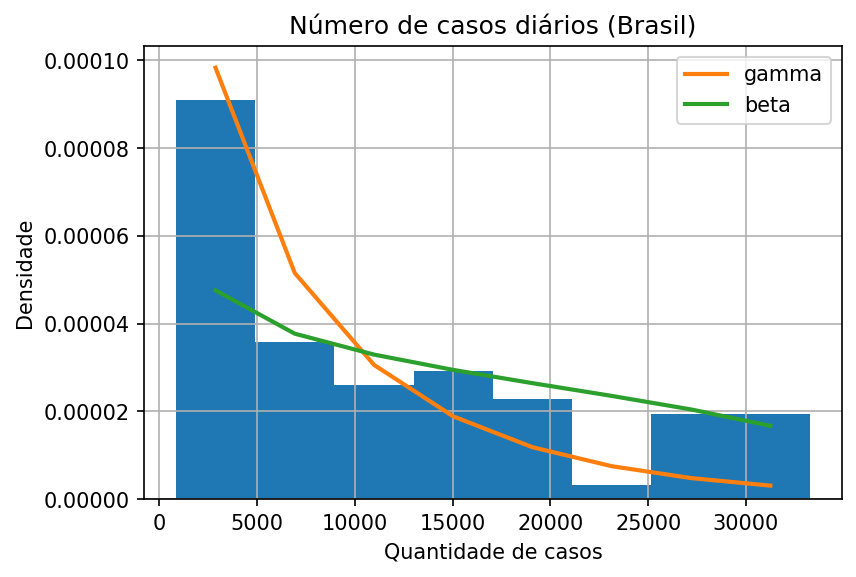
\includegraphics[height=6.2cm,width=6.5cm, frame]{images/pdfs/BRA_NDC.png}}}
\qquad
\subfloat[(b) NDM]{{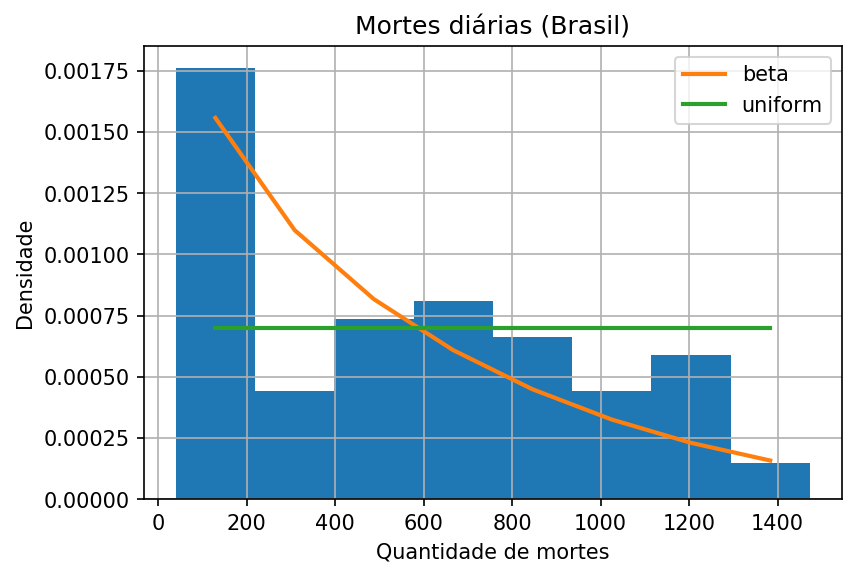
\includegraphics[height=6.2cm,width=6.5cm, frame]{images/pdfs/BRA_NDM.png}}}
\label{figure:pdf1}
\end{figure}

\par No atributo NDC, é possível perceber que, mesmo a PDF beta fazendo um ajuste, que de maneira geral segue a tendência dos dados, ao realizar o ajuste da PDF gama, o comportamento decrescente da distribuição dos dados é melhor representado. Isso ocorre já que, no ajuste beta, a curva decrescente da distribuição é pouco considerada, o que não ocorre na distribuição gama. Da mesma forma, para o atributo NDM, dos dois ajustes realizados é identificado a PDF beta como a melhor, seguindo o mesmo motivo apresentado para a variável NDC. O comportamento uniforme identificado no NDM, de certa forma, até faz a representação dos dados, porém, deixa de considerar as feições mais específicas, como ocorre nas quantidades entre 0 e 200.

\par O comportamento apresentado pelas distribuições do Brasil representam o crescimento que ambas as ocorrências tem apresentado, onde quantidades cada vez maiores de casos e mortes são registrados, dia após dia. Perceba que tais PDFs podem sofrer alterações e com o tempo passar para algo uniforme e em seguida ter um comportamento beta novamente, porém, com uma densidade concentrada à direita, nos valores maiores.

\par Nos dados do Canadá, em todos os atributos, múltiplas PDFs foram indicadas pelo ECF. No caso do NDC, das quatro indicações realizadas, três apresentam um bom ajuste aos dados, sendo a distribuição normal indicada como a melhor para este caso. Para o atributo NDM, a distribuição beta obteve melhor resultado, uma vez que, a distribuição normal e a uniforme deixam de considerar as características das caudas, que possuem valores que não podem ser representados por tais distribuições. No atributo de NDT, foi identificado e melhor ajustado uma distribuição normal, sendo condizente com a forma do fenômeno mapeado. Os ajustes são apresentados na Figura \ref{figure:pdf2} 

\begin{figure}[H]
\captionsetup[subfigure]{labelformat=empty}
\caption{Ajuste de PDF - Canadá}
\subfloat[(a) NDC]{{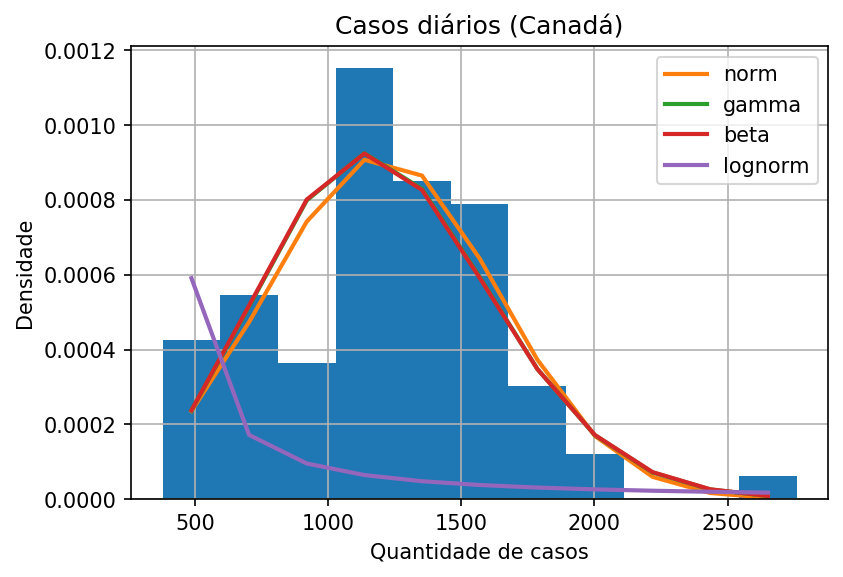
\includegraphics[height=6.2cm,width=6.5cm, frame]{images/pdfs/CAN_NDC.png}}}
\qquad
\subfloat[(b) NDM]{{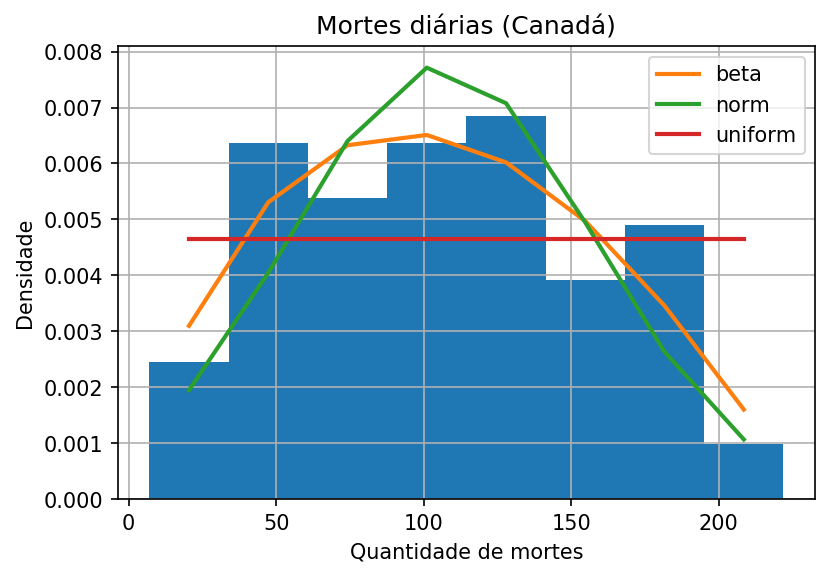
\includegraphics[height=6.2cm,width=6.5cm, frame]{images/pdfs/CAN_NDM.png}}}
\qquad
\centering
\subfloat[(c) NDT]{{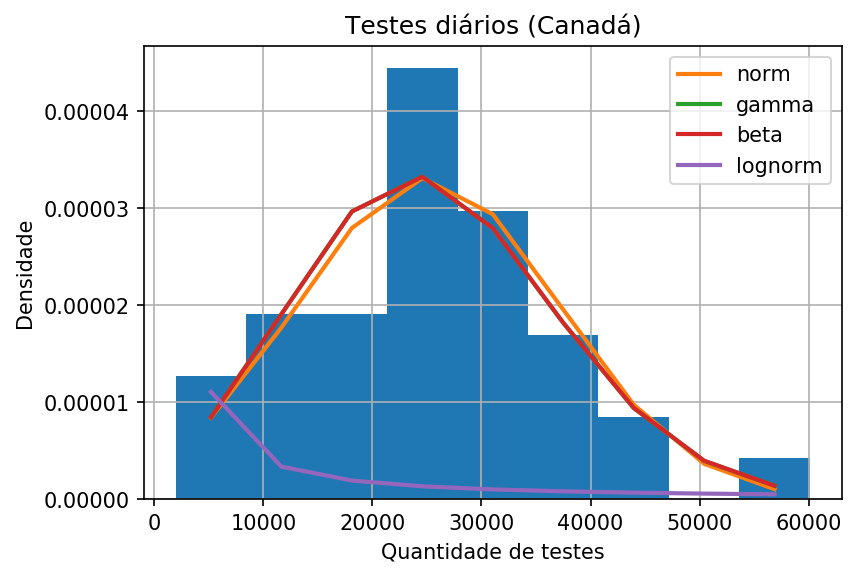
\includegraphics[height=6.2cm,width=6.5cm, frame]{images/pdfs/CAN_NDT.png}}}
\label{figure:pdf2}
\end{figure}

\par Com estes ajustes, fica evidente que as flutuações apresentadas pelo Canadá se mantiveram consistentes, o que pode ser vinculado ao controle feito pelo país frente a pandemia.

\par Diferente do ocorrido com o Canadá, para Cuba, que apresenta uma quantidade pequena de casos e mortes, em todos os atributos, foram identificados as PDFs beta, gama e uniforme, como apresentado na Figura \ref{figure:pdf3}. No atributo NDC, a distribuição beta representa bem o comportamento ao considerar os baixos valores com alta densidade, o que não ocorre com a distribuição uniforme. Nos atributos NDM e NDT, por conta das possibilidades que a distribuição beta pode assumir, a mesma foi considerada como o melhor ajuste em ambos os casos.

\begin{figure}[H]
\captionsetup[subfigure]{labelformat=empty}
\caption{Ajuste de PDF - Cuba}
\subfloat[(a) NDC]{{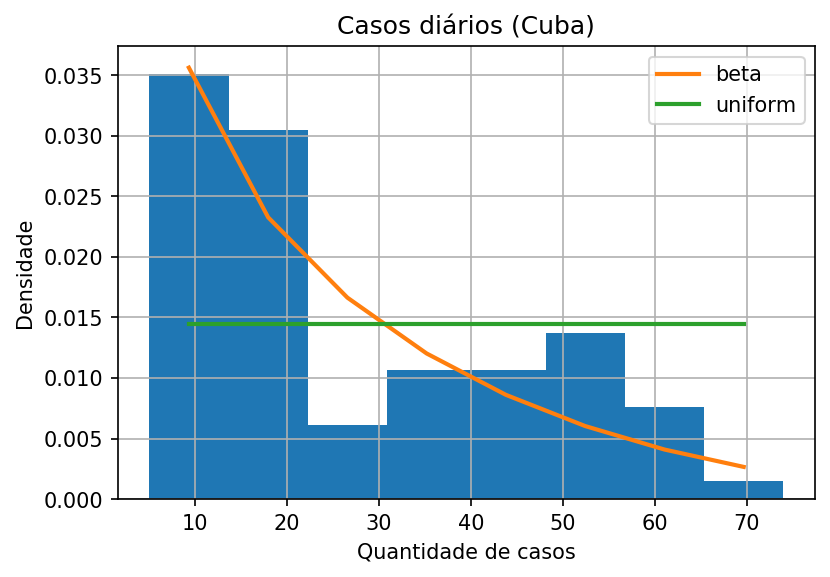
\includegraphics[height=6.2cm,width=6.5cm, frame]{images/pdfs/CUB_NDC.png}}}
\qquad
\subfloat[(b) NDM]{{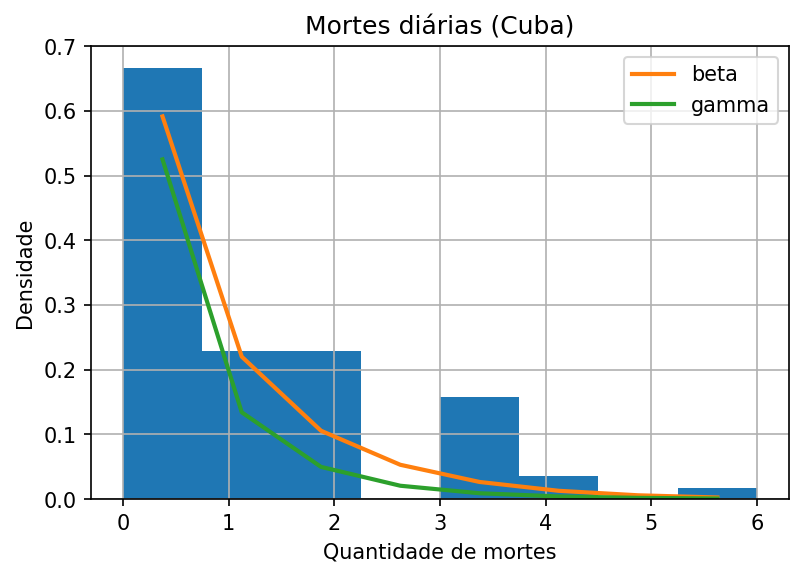
\includegraphics[height=6.2cm,width=6.5cm, frame]{images/pdfs/CUB_NDM.png}}}
\qquad
\centering
\subfloat[(c) NDT]{{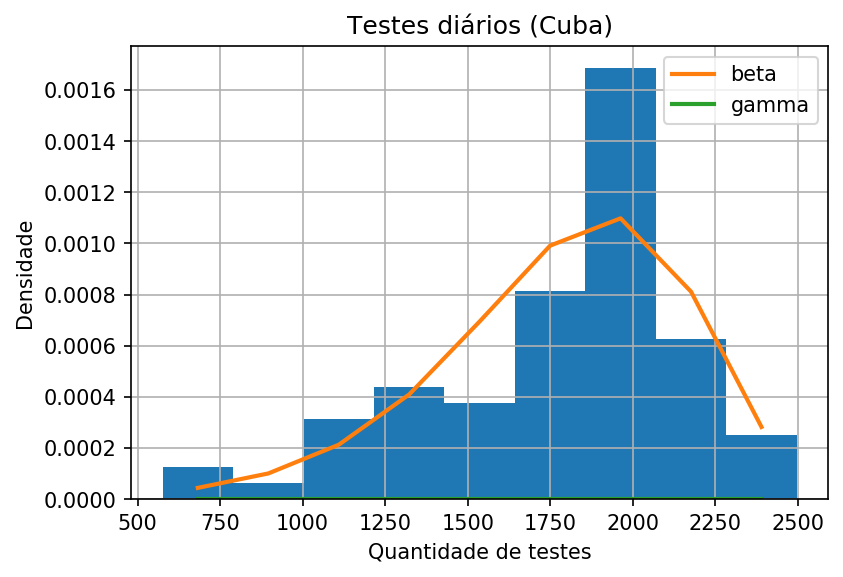
\includegraphics[height=6.2cm,width=6.5cm, frame]{images/pdfs/CUB_NDT.png}}}
\label{figure:pdf3}
\end{figure}

\par Vale notar que a maneira com que os dados estão dispostos, indicam uma boa resposta do país para a pandemia, onde a densidade das distribuições estão, em sua maioria, próximas aos baixos valores, sendo diferente apenas para os testes, que apresentam maior densidade ao lado das maiores quantidades.

\par Os ajustes realizados para os atributos do México foram feitos considerando as PDFs beta e uniforme, como na Figura \ref{figure:pdf4}, onde, o comportamento descrente da distribuição do NDM é completamente representado pela distribuição beta. Já para o NDC, a distribuição beta é utilizada, onde o mesmo comportamento apresentado no NDM do Brasil (Figura \ref{figure:pdf1} (b)), que, mesmo sendo indicado como uma distribuição uniforme, não pode ser representado por tal por conta dos comportamentos apresentados no início da distribuição dos dados, que tem muito mais representatividade na área de probabilidades que o restante.

\begin{figure}[H]
\captionsetup[subfigure]{labelformat=empty}
\caption{Ajuste de PDF - México}
\subfloat[(a) NDC]{{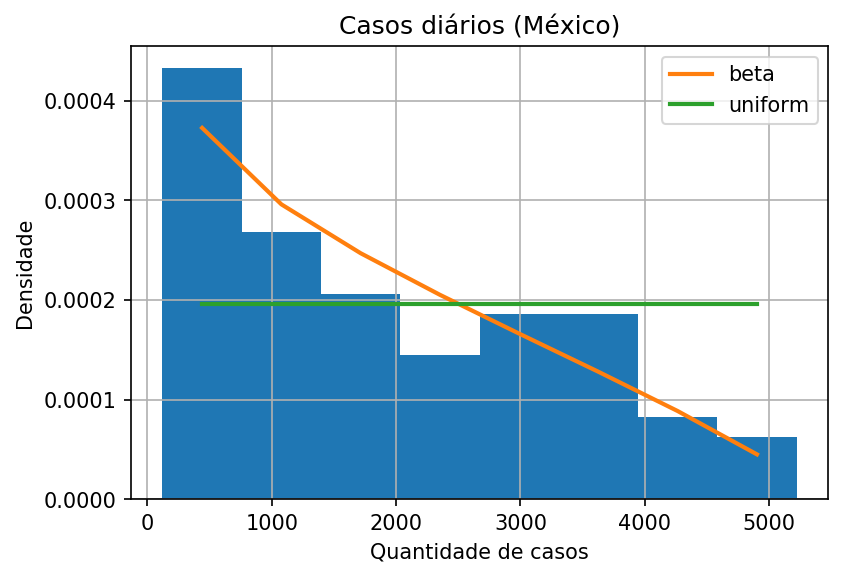
\includegraphics[height=6.2cm,width=6.5cm, frame]{images/pdfs/MEX_NDC.png}}}
\qquad
\subfloat[(b) NDM]{{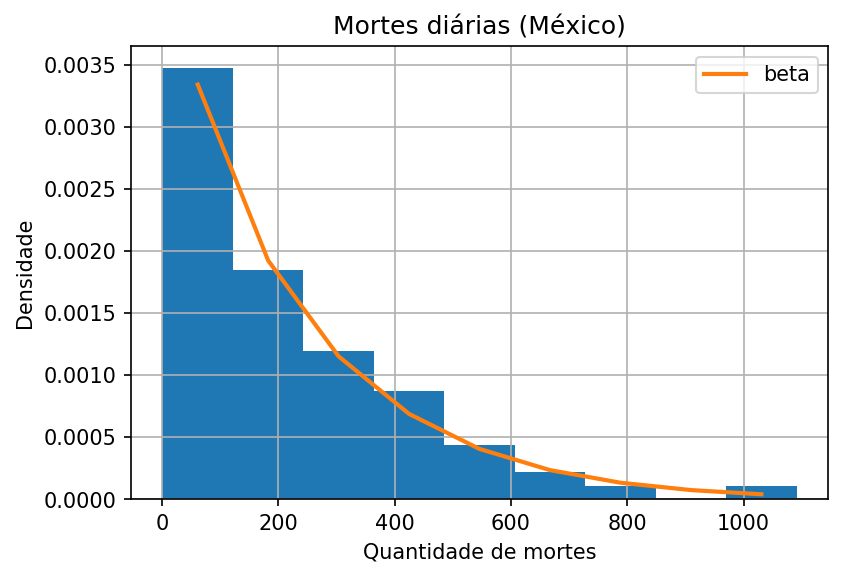
\includegraphics[height=6.2cm,width=6.5cm, frame]{images/pdfs/MEX_NDM.png}}}
\qquad
\centering
\subfloat[(c) NDT]{{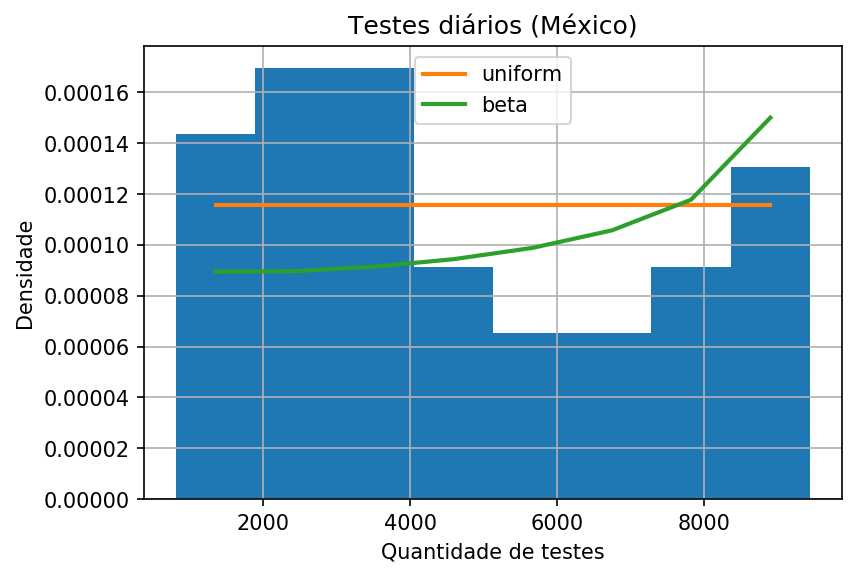
\includegraphics[height=6.2cm,width=6.5cm, frame]{images/pdfs/MEX_NDT.png}}}
\label{figure:pdf4}
\end{figure}

\par Veja que a distribuição do atributo NDC do México, ao ficar próxima de uma PDF uniforme apresenta comportamento semelhante ao identificado no Brasil (Figura \ref{figure:pdf1}), onde os valores maiores, representam cada vez mais área de probabilidade que os valores menores, o que pode vir a indicar uma crescente na quantidade de casos, porém, tal comportamento não é identificado no atributo NDM, que pelo contrário, mantém boa parte de seus valores concentrado nas menores faixas. Já no atributo NDT, diferente de todos os outros apresentados até aqui, tem-se uma distribuição com características que a fizeram ser representadas pela PDF uniforme.

\newpage % Temporário =D

\par Por fim, são feitas as considerações com os dados da Rússia, que durante os testes com o ECF foram indicadas várias PDFs. No atributo NDC, quatro ajustes foram feitos, porém, como pode ser notado na Figura \ref{figure:pdf5}, nenhuma delas conseguiu considerar por completo o comportamento dos dados, como pode ser observado nos demais países e atributos, isto, ocorre já que, o ECF é uma ferramenta utilizada como ponto de partida, não tratando ou representando todas as possíveis PDFs, isto indica que, outras mais poderia ser ajustadas de forma a diminuir os erros apresentados. Mesmo com tal característica, foi atribuído a este atributo a distribuição uniforme. De forma diferente a este comportamento, o atributo NDM é bem representado pela PDF beta, o que ocorre de maneira semelhante no NDT, com a diferença que este é representado pela PDF uniforme.

\begin{figure}[H]
\captionsetup[subfigure]{labelformat=empty}
\centering
\caption{Ajuste de PDF - Rússia}
\subfloat[(a) NDC]{{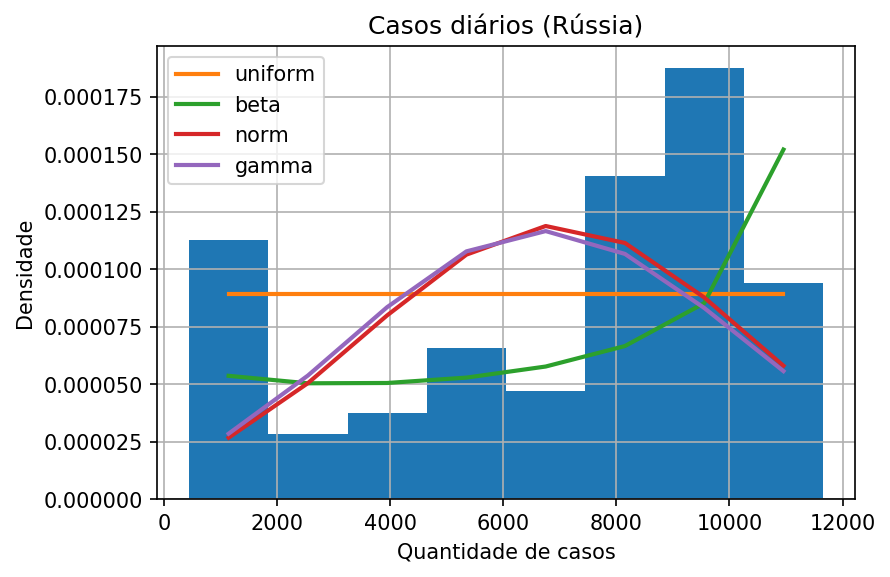
\includegraphics[height=6.2cm,width=6.5cm, frame]{images/pdfs/RUS_NDC.png}}}
\qquad
\subfloat[(b) NDM]{{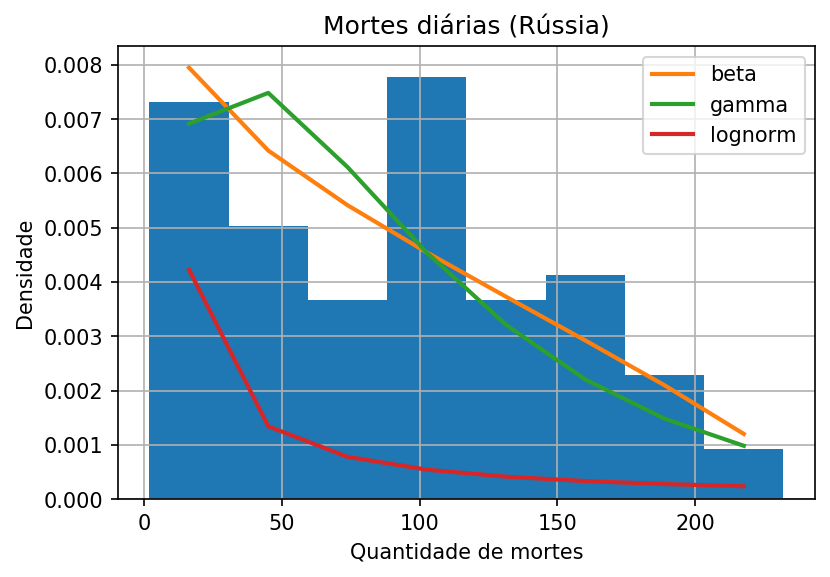
\includegraphics[height=6.2cm,width=6.5cm, frame]{images/pdfs/RUS_NDM.png}}}
\qquad
\subfloat[(c) NDT]{{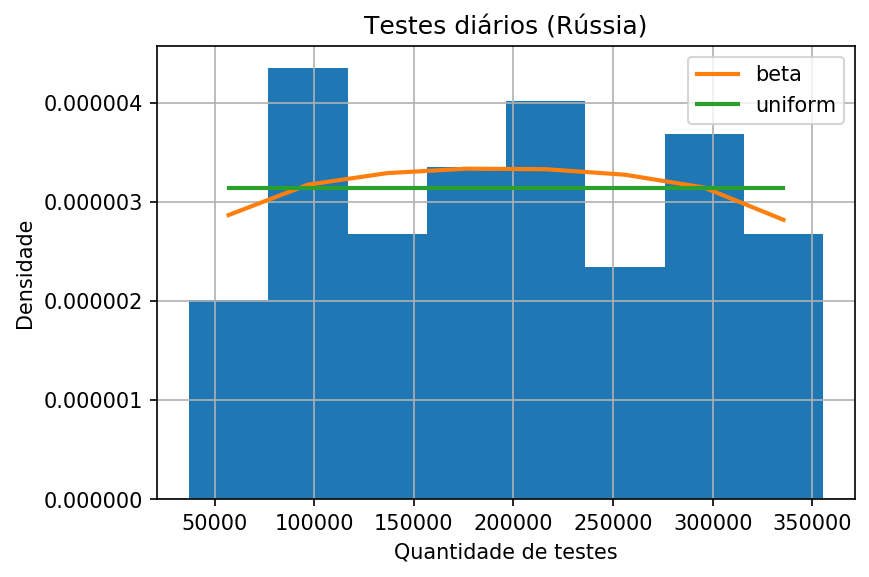
\includegraphics[height=6.2cm,width=6.5cm, frame]{images/pdfs/RUS_NDT.png}}}
\label{figure:pdf5}
\end{figure}

\par Assim, após a análise de cada um dos ajustes realizados é possível perceber que para boa parte dos comportamentos apresentados os ajustes indicados no ECF foram o suficiente para o ajuste mínimo aos dados, mas, há casos em que isto não ocorre, o que pode ser resolvido com uma análise mais profunda dos tipos de distribuição. Como forma de mapear tal comportamento, testes foram feitos considerando todas as distribuições do pacote\footnote{\href{https://www.scipy.org/}{SciPy.org}}. Os resultados são apresentados no repositório deste projeto.

\subsection{Identificação de similaridade}

\par Uma das várias etapas de de análise de dados é a identificação de comportamentos e similaridade no próprio conjunto de dados, o que ajuda no entendimento dos comportamentos e relações assumidas pelos fenômenos registrados. Nas seções anteriores, diferentes técnicas foram utilizadas para a busca de comportamentos dos dados, verificando sua distribuição e suas classes estatísticas, porém, na etapa de análise desses resultados, podem haver características que não foram consideradas ou notas. Desta forma, com o objetivo de identificar e mapear possíveis comportamentos presentes nos dados, 
é feita a aplicação do análise de agrupamento \textit{K-Means}. Para isto, cada uma das séries é sumarizada considerando as métricas de \texttt{curtose}, \texttt{assimetria} e \texttt{variância}. 

\par Dentro os passos para a aplicação do \textit{K-Means} está a identificação do melhor valor de $K$, este que será utilizado para definir a quantidade de grupos criados durante o agrupamento. Em um fluxo padrão de aplicação, esta etapa seria resolvida com métodos como \textit{Elbow} e \textit{Silhouette}, que fazendo avaliações nos grupos gerados com diferentes valores de $K$ e com auxílio de uma função objetivo, definem o melhor valor de $K$ a ser aplicado, porém, neste caso, o conjunto de dados com tamanho limitado faz com que tais técnicas não apresentem bons comportamentos e não ajudem na identificação dos valores de $K$. Com isso, para a aplicação do método, fez-se a consideração da variação dos valores de $K$ dentro do intervalo $[2, 4]$. Este intervalo foi definido seguindo o critério de que, com apenas um grupo e com cinco grupos, não há nenhum agrupamento feito, uma vez que o objetivo é juntar elementos semelhantes.

\par Para a aplicação da análise de agrupamento, considerou-se os atributos NDC e NDM, por estas serem as únicas que apresentam flutuações, como já informado e por estarem presentes em todas séries do conjunto, uma vez que, para os valores de NDT por exemplo, países como o Brasil não possuem dados. Foram desenvolvidas três baterias de testes, cada uma delas considerando a variação dos valores de $K$ e do atributo considerado. Cada uma das baterias de testes são apresentadas nas subseções abaixo.

\subsubsection{Avaliação dos grupos com o atributo NDC}

\par Para o primeiro teste foi realizada o agrupamento dos dados considerando o uso do atributo NDC com o valor de $K $ = 3. O resultado do agrupamento é apresentado na Figura  \ref{figure:group_ndc}, onde é possível perceber que o Brasil e a Rússia apresentam comportamentos que acabam sendo diferentes dos apresentados pelos demais países analisados. Ao conferir as características de cada um dos grupos, percebe-se que para um destes dois casos, que ficaram em grupos separados, há valores de variância muito diferente dos demais grupos, o que faz com que, mesmo outras características sendo próximas as demais séries, estes fiquem em grupos isolados dos demais.

\image{0.9}{images/analise_de_agrupamento/1_grupos_k3_ndc.png}{Agrupamento pelo número diário de casos}{figure:group_ndc}

\par Para este resultado vale notar que, mesmo considerando que o \textit{K-Means} precisa realizar a classificação de cada uma das séries de dados em um grupo, o que pode, a priori ser indicado como apenas um viés do método, considera-se que se tais grupos não fossem tão discrepantes dos demais, eles poderia estar agrupados juntos, dado que sua proximidade os relacionaria e possivelmente outros países tomariam os grupos específicos

\subsubsection{Avaliação dos grupos com o atributo NDM}

\par Diferente dos resultados da análise feita anteriormente, para o caso do atributo NDM, tem-se que o México e o Brasil apresentam características discrepantes aos demais membros, o que faz estes serem inseridos em grupos separados dos demais, como apresentado na Figura \ref{figure:group_ndm}

\image{0.9}{images/analise_de_agrupamento/1_grupos_k3_ndm.png}{Agrupamento pelo número diário de mortes}{figure:group_ndm}

\par Vale considerar também que, neste caso, o valor de variância encontrado também difere entre os elementos que ficaram em grupos separados dos demais, assim como encontrado no teste anterior. Assim como levantado no teste anterior, a ideia de que, mesmo existindo a necessidade de definição de uma série para cada grupo, fica evidente que os países isolados, possuem características que evitam que estes sejam postos em grupos com outros elementos, como acontece com o Canadá e a Rússia.

\subsubsection{Avaliação dos grupos com os atributos NDC e NDM}

\par Como forma de considerar os dois atributos avaliados anteriormente em uma única análise de agrupamento, esta seção apresenta os testes e avaliação dos resultados obtidos ao realizar o agrupamento considerando estes dois atributos simultaneamente. Para este caso, foi decidido que os agrupamentos realizados serão feitos considerando a variação de $K$ em todos os valores do intervalo apresentado anteriormente. O primeiro teste, feito com valor de $K$ = 2  é apresentado na Figura \ref{figure:group_ndcndm1}, neste é possível notar que o Brasil, mesmo tendo iniciado as curvas da pandemia junto a outros países que estão sendo analisados, como o Canadá, fica isolado dos demais.

\image{0.9}{images/analise_de_agrupamento/2_grupos_k2_ndc-e-ndm.png}{Agrupamento pelo número diário de casos e mortes ($K$ = 2)}{figure:group_ndcndm1}

\par Para este caso, o valor pequeno de $K$ foi definido com o objetivo de identificar o elemento que possuí as características mais discrepantes dentre todos os países que estão sendo analisados. Por outro lado, ao colocar o valor de $K$ = 3, percebe-se o mesmo comportamento já apresentado nos casos de testes anteriores, onde, o Brasil e a Rússia ficam separados dos demais elementos do conjunto de dados.

\image{0.9}{images/analise_de_agrupamento/2_grupos_k3_ndc-e-ndm.png}{Agrupamento pelo número diário de casos e mortes ($K = 3$)}{figure:group_ndcndm2}

\par Por fim, é feita a análise considerando o valor de $K = 4$, para esta, o interessante é notar que, o México, que no segundo teste ficou isolado junto ao Brasil, acabou ficando também em um grupo separado.

\image{0.9}{images/analise_de_agrupamento/2_grupos_k4_ndc-e-ndm.png}{Agrupamento pelo número diário de casos e mortes ($K = 4$)}{figure:group_ndcndm3}

\par Com estes testes foi possível identificar que, dentre todos os países analisados neste trabalho, o que apresenta as características mais discrepantes é o Brasil, estando separado de todos os demais em todos contextos de testes realizando, isso ocorrendo em ambas as variáveis. Tal comportamento não é identificado em outros países, uma vez que na baixa quantidade de valores de $K$, semelhança entre todos os demais países, menos que mínima fez com que os mesmos fossem colocados em grupos iguais.

\subsection{Análise de regressão}

\par A análise de regressão avalia a amplitude da variação em uma variável, decorrente da variação em outra variável. Isto é, consiste na realização de uma análise estatística com o objetivo de verificar a existência de uma relação funcional entre duas variáveis. Logo, um modelo de regressão linear serve para prever comportamentos com base na associação entre duas variáveis que geralmente possuem uma boa correlação. Sendo assim, foi realizada neste estudo uma análise de regressão linear entre as variáveis NDC e NDT para cada país, com exceção do Brasil, que não possui dados de testes diários. Serão apresentados também os coeficientes de  \texttt{Correlação} e \texttt{Determinação}, associados à quanto as variáveis estão relacionadas entre si e quanto a regressão linear representa a distribuição dos dados, respectivamente. 

\par Começando com o México, (Figura \ref{figure:reg_mex}), nota-se que coeficiente de correlação entre as duas variáveis fica em torno de 0.5. Pode-se especular com isso que a variação no número de casos esta relacionado em 50\% ao aumento do número de testes e 50\% ao próprio aumento de pessoas infectadas. Já o coeficiente de determinação calculado indica que a regressão linear obtida tem baixa representatividade do conjunto de dados. 

\image{0.79}{images/regressao_linear/regressao_linear_NDCxNDT_MEX}{Regressão Linear Numero de Casos x Numero de Testes (México)}{figure:reg_mex}

\par Para a Rússia (Figura \ref{figure:reg_rus}) é possível observar que o coeficiente de correlação foi mais alto que o México, ficando em torno de 0.69, indicando que a hipótese de que quanto mais testes realizados, maior o número de casos identificados. É interessante reparar neste caso que, embora o coeficiente de correlação não tenha sido muito alto, a reta obtida pela regressão linear consegue captar a tendência de evolução das variáveis. 

\image{0.79}{images/regressao_linear/regressao_linear_NDCxNDT_RUS}{Regressão Linear Numero de Casos x Numero de Testes (Rússia)}{figure:reg_rus}

\par O caso de Cuba (Figura \ref{figure:reg_cub}) pode ser considerado como exemplo de país onde o número de casos identificados não está relacionado ao número de testes realizados, ou seja, mesmo realizando mais testes, não foi registrado aumento notável no número de infectados. Os coeficientes convergem para isto, sendo muito próximos de zero, ou seja, não indicam correlação entre as variáveis, nem mesmo a regressão linear consegue representar a distribuição dos dados.

\image{0.79}{images/regressao_linear/regressao_linear_NDCxNDT_CUB}{Regressão Linear Numero de Casos x Numero de Testes (Cuba)}{figure:reg_cub}

\par Por fim, o Canadá (Figura \ref{figure:reg_can}) apresentou coeficiente de correlação levemente negativo, indicando de forma subjetiva que apesar de quase nula a relação entre o número de casos e o número de testes, aumentando o número de testes realizados, houve uma leve queda no número de infectados registrados. Quanto ao coeficiente de determinação, nota-se que ele é extremamente baixo, o que indica que a regressão linear não foi capaz de representar o conjunto de dados. 

\image{0.79}{images/regressao_linear/regressao_linear_NDCxNDT_CAN}{Regressão Linear Numero de Casos x Numero de Testes (Canada)}{figure:reg_can}

\par Logo, a regressão linear aplicada para os países deste grupo indica que o fato de aumentar a quantidade de testes realizados em um dia não necessariamente irá fazer com que haja aumento no número de casos registrados. 

\subsection{Criticalidade auto-organizada}

\par Identificações de assinatura SOC podem ser feitas em qualquer conjunto de dados, exigindo apenas que este tenha disponível grandes quantidades de amostras. Com isso, a caracterização de SOC no conjunto de dados criado para este trabalho torna-se inviável sem a aplicação de métodos para o aumento do conjunto de amostras. Desta forma, para o o aumento de dados, fez-se a aplicação de interpolações aleatórias nas séries de dados. Neste caso, foi feita a implementação de dois tipos diferentes de interpolação aleatória, uma discreta, nomeada de \texttt{Método por inteiros} e outra contínua, nomeada de \texttt{Método dos polinômios}. 

\par A forma de funcionamento de cada um dos métodos é semelhante, onde, dado um intervalo entre duas datas, faz-se a divisão deste intervalo em $N$ intervalos $h$ e para cada um desses atribui-se um valor. A diferença está somente na maneira com que esta atribuição de valores ocorre. Para o caso do \texttt{Método por inteiros}, valores inteiros aleatórios são gerados e atribuídos à cada intervalo $h$. Já no \texttt{Método dos polinômios}, faz-se primeiro o ajuste de um polinômio entre os valores de duas datas, em seguida, este polinômio é utilizado para gerar os valores de cada intervalo $h$. A representação de cada um desses métodos é feita na Figura \ref{figure:randominterpmethods}.

\image{1.05}{images/interpolacao/interp_geral.svg.png}{Métodos de interpolação aleatória}{figure:randominterpmethods}

\par No método de inteiros, a série temporal gerada é pode ser representada como apresentado na Figura \ref{figure:interp1d1}. Perceba que a série mantém o mesmo formato, porém com um sinal mais grosso, representando múltiplos valores dentro de um intervalo. Neste caso, para cada intervalo entre duas datas é inserido 23 valores, criando a representação das horas.

\image{0.80}{images/interpolacao/exemplos/interp_inteiros.png}{Método de interpolação aleatória com valores inteiros}{figure:interp1d1}

\par Por outro lado, na Figura \ref{figure:interp1d2} tem-se a apresentação do método por polinômios, onde o sinal aparentemente é o mesmo, isso ocorrendo por conta da natureza contínua dos elementos gerados, o que pode representar uma variação não muito grande dos elementos que estão dentro do conjunto pode ocorrer.

\image{0.80}{images/interpolacao/exemplos/interp_polinomios.png}{Método de interpolação aleatória com valores contínuos}{figure:interp1d2}

\par Com estes métodos de interpolação criados, fez-se o aumento de dados de cada uma das séries temporais que constituem o conjunto de dados deste trabalho e então a assinatura SOC pode ser verificada. Como exemplo de resultado desta operação, tem-se os dados de Cuba, que seu o aumento de dados, apresentada algo que não tinha uma boa representação de SOC, como apresentado na Figura \ref{figure:soc_1}.

\image{0.85}{images/soc/pais/soc_cuba_nointerp.png}{Assinatura SOC para os dados de Cuba sem interpolação}{figure:soc_1}

\par Por outro lado, ao aplicar a interpolação, uma possível assinatura SOC é apresentada (Figura \ref{figure:soc_2}). Para este caso o método de inteiros foi aplicado, porém, o método de polinômios poderia ser aplicado também.

\image{0.85}{images/soc/pais/soc_cuba.png}{Assinatura SOC para os dados de Cuba com interpolação}{figure:soc_2}

\par Vários outros testes foram realizados e estão disponíveis no repositório deste projeto.

\section{Predição de casos diários}

\par A realização de predições e identificação de comportamentos que as séries temporais vão tomar são extremamente úteis para as mais variadas aplicações. Ao considerar o contexto de aplicação deste Trabalho, este fato não é diferente. Com a previsão e estimativa de comportamentos futuros de novas infecções diárias, decisões podem ser tomadas, pelas instituições públicas e privadas de forma a evitar que possíveis alastres e aumento dos infectados pela doença sejam causados, o que ajuda na preservação da vida. Esta seção apresenta duas técnicas que foram aplicadas neste estudo com o objetivo de prever a quantidade de casos diários em diferentes quantidades de dias no futuro. Para isto, aplicam-se as técnicas de Rede Neural \textit{Long Short-Term Memory} (LSTM) e também um modelo de cascata multiplicativa baseado em fluídos sociais.

\subsection{Rede Long short-term memory}

\par Redes Neurais Recorrentes (RNN) são tipos específicos de redes neurais, que possuem a capacidade de armazenar estados processados em tempos anteriores, para que, esses sejam usados na geração e identificação de valores futuros. Um tipo de RNN muito comum são as LSTM que com diferentes quantidades de unidades de memória, permitem a identificação de valores futuros considerando grandes quantidades de valores do passado. Para esta Seção, faz-se a aplicação do modelo de LSTM desenvolvido e disponibilizado pelo Luis Arantes Filho.

\par Para a utilização da LSTM, fez-se a criação de uma camada de abstração para a fácil utilização dos módulos e do modelo já implementados. Esta camada de abstração foi criada seguindo o padrão de projetos \textit{Facade}, que através de uma interface única, permite acesso a todas as funcionalidades do código base, de modo que, todas as configurações necessárias para a utilização do código base sejam feitas por esta camada de abstração.

\par A aplicação da LSTM neste trabalho teve por objetivo fazer a previsão de 7 dias a frente do dia atual, considerando diferentes quantidades de dias passados. Isto é feito como uma forma de identificar a possibilidade desde tipo de técnica ser aplicado em tomadas de decisões semanais, de modo que essas podem ser utilizadas em políticas públicas e privadas mais maleáveis, de forma a evitar um aumento na quantidade de infectados por conta de decisões tomadas sem as devidas verificações e previsões. 

\par Assim, com o objetivo de identificar a melhor combinação entre épocas de treinamento e a quantidade de dias passados considerados pela LSTM para a previsão dos 7 dias futuros, fez-se a implementação de diferente baterias de testes, estas suportadas pelo \textit{Facade} citado anteriormente. Nestas baterias de testes são feitas as variações entre grupos de configuração de quantidades de entrada e saída da rede e as épocas.  Para estes grupos de entradas e saídas foram considerados os seguintes elementos, $[(10, 7), (20, 7), (30, 7)]$, onde o primeiro elemento de cada tupla representa a quantidade de dias passados e o segundo elemento a quantidade de dias previstos, de modo que, para cada uma das tuplas identificadas, fez-se a geração de um modelo considerando as épocas 10, 50 e 100. A escolha pelo melhor modelo foi feita considerando o \textit{Root Mean Square Error} (RMSE) gerado por cada um dos modelos.

\par Para este documento, apenas os resultados gerados com os dados do Brasil serão apresentados, porém, no repositório do projeto há outros testes realizados considerando as diferentes regiões do Brasil. Com isto, depois da execução de vários testes para o conjunto de dados do Brasil, fez-se a escolha do modelo com o ajuste apresentado na Figura \ref{figure:lstm_1}. Perceba que neste, o comportamento gerado pela rede, não é idêntico, o que é o esperado, uma vez que, o objetivo principal da aplicação deste tipo de rede é a generalização do resultado e não, o acerto total a forma dos dados utilizados no treinamento, o que poderia ser indicado como \textit{Overfitting} do modelo. Os ajustes foram feitos considerando os dados de 31/12/2019 à 17/06/2020.

\image{0.85}{images/lstm/modelo_ajustado/1_modelo_ajustado_brasil.png}{Resultado do modelo de LSTM ajustado}{figure:lstm_1}

\par Após esta seleção do melhor modelo, fez-se a aplicação do mesmo para a previsão da quantidade de casos diários dos 7 dias após o dia 17/06/2020. O resultado é apresentado na Figura \ref{figure:lstm_2}.

\image{0.85}{images/lstm/previsao_realizada/1_predicao_brasil.png}{Resultado do modelo de LSTM ajustado}{figure:lstm_2}

\par Perceba, que o comportamento gerado pelo modelo segue as tendências que já estavam sendo apresentadas pelos dados, com tais informações, possíveis decisões sobre a maneira com que a pandemia está sendo tratada podem ser tomadas, como citado anteriormente.

\subsection{Modelo de cascatas multiplicativas}

\par Neste trabalho, como já citado, além do modelo de LSTM aplicado, fez-se também a implementação e aplicação do modelo desenvolvido e disponibilizado pelo Professor Doutor Reinaldo Rosa.  O modelo é baseado em cascatas multiplicativas não-homogêneas, que utiliza como entrada a média de novos casos dos sete dias anteriores ($\langle{N_{nb}}_7$) e o valor do dia atual ($N_{kt}$) para prever o dia seguinte ($N_s$) ao $N_{kt}$. A equação mestre do modelo pode ser definida como apresentado abaixo.

\begin{equation} 
N_{s_{min}}\:=\:g\:\left(1\:\cdot \:n_1+3\cdot n_2+5\cdot n_3\right)
\label{eq1}
\end{equation}

\begin{equation} 
N_{s_{max}}\:=\:g\:\left(2\:\cdot \:n_1+4\cdot n_2+6\cdot n_3\right)
\label{eq2}
\end{equation}

\par Onde $N_{s_{min}}$ e $N_{s_{max}}$, representam, respectivamente, os valores mínimos e máximos de possíveis infectados para o dia a ser predito. Para isto,

\begin{equation} 
n_1=p_1\cdot N_{kt}
\label{eq3}
\end{equation}

\begin{equation} 
n_2=p_2\cdot N_{kt}
\label{eq4}
\end{equation}

\begin{equation} 
n_3=p_3\cdot N_{kt}
\label{eq5}
\end{equation}

\par e

\begin{equation}
g\:=\:\frac{\left\langle N_{nb}\right\rangle _7}{N_{kt}},\:se\:N_{kt}\:>\left\langle N_{nb}\right\rangle _7
\label{eq6}
\end{equation}

\begin{equation}
g\:=\:\frac{N_{kt}}{\left\langle N_{nb}\right\rangle _7},\:se\:N_{kt}\:<\left\langle N_{nb}\right\rangle _7
\label{eq7}
\end{equation}

\par O modelo também calcula o fator de supressão, $s(t)$, baseado nas derivativas de g: $\Delta_g$ e n: $\Delta_{nk}$, onde, o $\Delta_g$ pode ser definido como:

\begin{equation}
\Delta _g=\left(g_0-g\right)-q_g,\:\:se\:\:g_0\:<\:g
\label{eq8}
\end{equation}

\begin{equation}
\Delta _g=\left(g_0-g\right)+q_{g0},\:\:se\:\:g_0\:\ge \:g
\label{eq9}
\end{equation}

\par Assim, o derivativo de $\Delta_{nk}$ é definido como:

\begin{equation}
\Delta _{nk}=\frac{\left(\left\langle N_{nb}\right\rangle _7-N_{kt}\right)}{N_{kt}}
\label{eq10}
\end{equation}

\par Onde,

\begin{equation}
s\:=\:\frac{2\Delta _g+\Delta _{nk}}{3}
\label{eq10}
\end{equation}

\par Vale notar que, mesmo com a descrição do modelo feita acima, o valor de $s$ apresentado nos resultados abaixo está sendo calculado como descrito na Equação \ref{eq11}.

\begin{equation}
s\:=\:1-g
\label{eq11}
\end{equation}

\par Com isto, para testar a implementação realizada, foram gerados casos de testes para todas as localidades que estão sendo analisadas neste trabalho. As subseções abaixo, porém, apresentam dois destes casos de teste, onde são considerados os dados do Estado de Minas Gerais e os dados gerais do Brasil. Os demais testes estão listados e documentados no repositório do projeto. Todos os testes foram desenvolvidos considerando o período de 08/04/2020 à 28/04/2020, uma vez que, o comportamento crescente do modelo, fez com que, a aplicação do mesmo neste trabalho, fosse feita de modo a considerar intervalos de predição.

\par Para a realização de um comparativo da quantidade de elementos que foram estimadas pelo modelo são consideradas as quantidades de possíveis novos casos diários estimados pela Fiocruz.

\subsubsection{Dados gerais do Brasil}
\label{sssectionBrasil}

\par Para começar, os testes com os dados do Brasil, fez-se a predição dos casos considerando o espectro de peso 1. O resultado apresentado na Figura \ref{figure:model_country1}, mostra o comportamento geral de previsão do modelo implementando ao considerar tal espectro de pesos. O comportamento, indica uma crescente contínua, de forma exponencial, do crescimento do número de casos diários no Brasil, porém, vale ressaltar que, o comportamento do modelo, como apresentado anteriormente, considera fatores de sub-notificação.

\image{0.85}{images/modelo/pais/estimativa_Brasil_1.png}{Resultados do modelo com o 1° espectro de pesos}{figure:model_country1}

\par Durante este teste, para o valor de $g$, tem-se que o mesmo variou dentro de um intervalo positivo, passando a ter uma baixa variação após algumas iterações do modelo. Por outro lado, os valores do parâmetro $s$ mantiveram um padrão de variação durante toda a simulação de predição realizada, como visto na Figura \ref{figure:model_country1gs}.

\image{0.75}{images/modelo/pais/gs_modelo_Brasil_1.png}{Variação dos parâmetros $g$ e $s$ com espectro de peso 1}{figure:model_country1gs}

\par Após a finalização deste primeiro teste de previsão dos casos diários, um segundo teste foi realizado, este considerando o espectro de peso 2 (Figura \ref{figure:model_country2}). Os resultados, diferente do apresentado anteriormente, apresentam um crescimento contínuo, porém, em passos menores e mais suaves, garantindo que a previsão acompanhe a tendência das notificações de casos reais. Este comportamento torna evidente a capacidade do modelo de identificar as sub-notificações presentes nos dados, mantendo-se próximo aos valores estimados pela Fiocruz.

\image{0.85}{images/modelo/pais/estimativa_Brasil_2.png}{Resultados do modelo com o 2° espectro de pesos}{figure:model_country2}

\par Para os parâmetros $g$ e $s$, é percebido um comportamento igual ao levantado anteriormente, com a diferença de que as variações ocorrem em um intervalo de valores menor.

\image{0.75}{images/modelo/pais/gs_modelo_Brasil_2.png}{Variação dos parâmetros $g$ e $s$ com espectro de peso 2}{figure:model_country2gs}

\subsubsection{Dados do Estado de Minas Gerais}

\par Para a avaliação do comportamento do modelo, foi criada uma segunda bateria de testes, esta considerando os dados do Estado de Minas Gerais, os passos tomados aqui seguem o mesmo padrão dos testes realizados para o conjunto de dados completo do Brasil, com isto, inicialmente faz-se a aplicação do modelo considerando o 1° espectro de pesos e da mesma maneira como apresentado no teste anterior, o comportamento das previsões feitas pelo modelo com estes espectros de peso acabam sendo muito diferentes da realizada, obtendo comportamento de crescimento exponencial.

\image{0.85}{images/modelo/regiao/estimativa_MG_1.png}{Resultados do modelo com o 1° espectro de pesos}{figure:model_region1}

\par Neste teste, os valores de $g$ e $s$, como pode ser observado na Figura \ref{figure:model_region1gs}, possuem o comportamento similar ao apresentado na Figura \ref{figure:model_country1gs}, sendo diferente somente nas escalas de variação. 

\image{0.75}{images/modelo/regiao/gs_modelo_MG_1.png}{Variação dos parâmetros $g$ e $s$ com espectro de peso 1}{figure:model_region1gs}

\par Ao considerar o 2° espectro de pesos para estes dados, o mesmo comportamento observado na Seção \ref{sssectionBrasil} é apresentado, onde uma curva que se ajusta de maneira muito mais clara a realizada é gerada. 

\image{0.85}{images/modelo/regiao/estimativa_MG_2.png}{Resultados do modelo com o 2° espectro de pesos}{figure:model_region2}

\par Nos parâmetros $g$ e $s$ comportamentos similares ao observado na Figura \ref{figure:model_country2gs} são identificados.

\image{0.75}{images/modelo/regiao/gs_modelo_MG_2.png}{Variação dos parâmetros $g$ e $s$ com espectro de peso 2}{figure:model_region2gs}

\par Com isto, pode-se concluir que, os espectros de peso 2 apresentam melhor comportamento, o que pode indicar que este representa melhor a maneira com que as transmissões do vírus ocorrem, porém, vale notar que, para a implementação realizada do modelo problemas com predições de longa escala foram identificados, uma vez que o comportamento de convergência da variável $g$ faz com que a curva permaneça constante, o que pode não representar por completo a pandemia de determinadas regiões e países.

\section{Conclusão}

\par Após a realização e aplicação das diferentes técnicas estatísticas para a análise dos dados, fica claro que, mesmo com um conjunto de ferramentas simples é possível extrair diversas informações dos dados. Além disto, a caracterização realizada neste trabalho, indica que do conjunto de países analisados, Canadá e a Rússia apresentam os melhores comportamentos frentes a pandemia que está sendo enfrentada.

% \newpage
% \bibliographystyle{acm}
% \bibliography{bibfile}

\end{document}
